
\section{Background}
\label{sec:background}
This section will focus on describing the fundamental principles behind our voice conversion algorithm. It will describe human voice differentiation, the human auditory response in conjunction with the mel frequency bank and Mel cepstrums, the Dynamic Time Warping algorithm, and a description of Gaussian Mixture Models.
\subsection{Human Voice Production and Identification}

Unfortunately for voice conversion technology, speakers have a variety of individual characteristics that affect their speech. Human vocal tract and speaking patterns are highly individualized and humans have evolved a strong ability to discriminate between different speakers \cite{latinus2011human}.  Speaking rate, pitch contour, etc are all important features that help to identify individual speakers. However, some of the most significant characteristics of speaker identity are embedded in the statistical distribution of the speech envelope\cite{reynolds1995robust}. Based on this concept and previous work, we will focus on voice conversion using the speech envelope as our primary feature.

Of additional importance is the distinction between ``voiced'' and ``unvoiced'' frequencies. Voiced sounds are produced by vocal cords, have more amplitude, and can be represented by near-constant frequencies of a particular duration. The maximum voiced frequency tends to be cut off at about 4 kHz. Above this range, there are ``unvoiced'' sounds, which are non-periodic sounds caused by air pressed through a constricted vocal tract. Due to the aperiodic and short-time nature of such events, they tend to have more frequency components which also tend to be higher\cite{bachu2008separation}. Studies have shown voiced speech to play a larger role in speaker individuality than unvoiced speech \cite{stylianou1998continuous}, so our conversion will focus on the voiced portions of speech.

\subsection{Human Auditory Response and the Mel Frequency Bank}
Human auditory response further complicates analysis and reconstruction of speech. Specifically, human perception of pitch, or frequency, follows a nonlinear scale. When humans judge whether pitches are equal distances from one another, they select frequencies over larger and larger intervals, starting around 500 Hz. In addition, the same sound amplitude over a range of frequencies will have different perceived loudness levels over those frequencies. Based on these phenomenon, the Mel scale was developed\cite{ghosh2012comparative}. A Mel-filter bank can be created to simulate the filtering occurring in the human auditory system with a series of overlapping triangular bandpass filters, centered on the Mel frequencies. 
\begin{figure}[htb]

\begin{minipage}[b]{1.0\linewidth}
  \centering
  \centerline{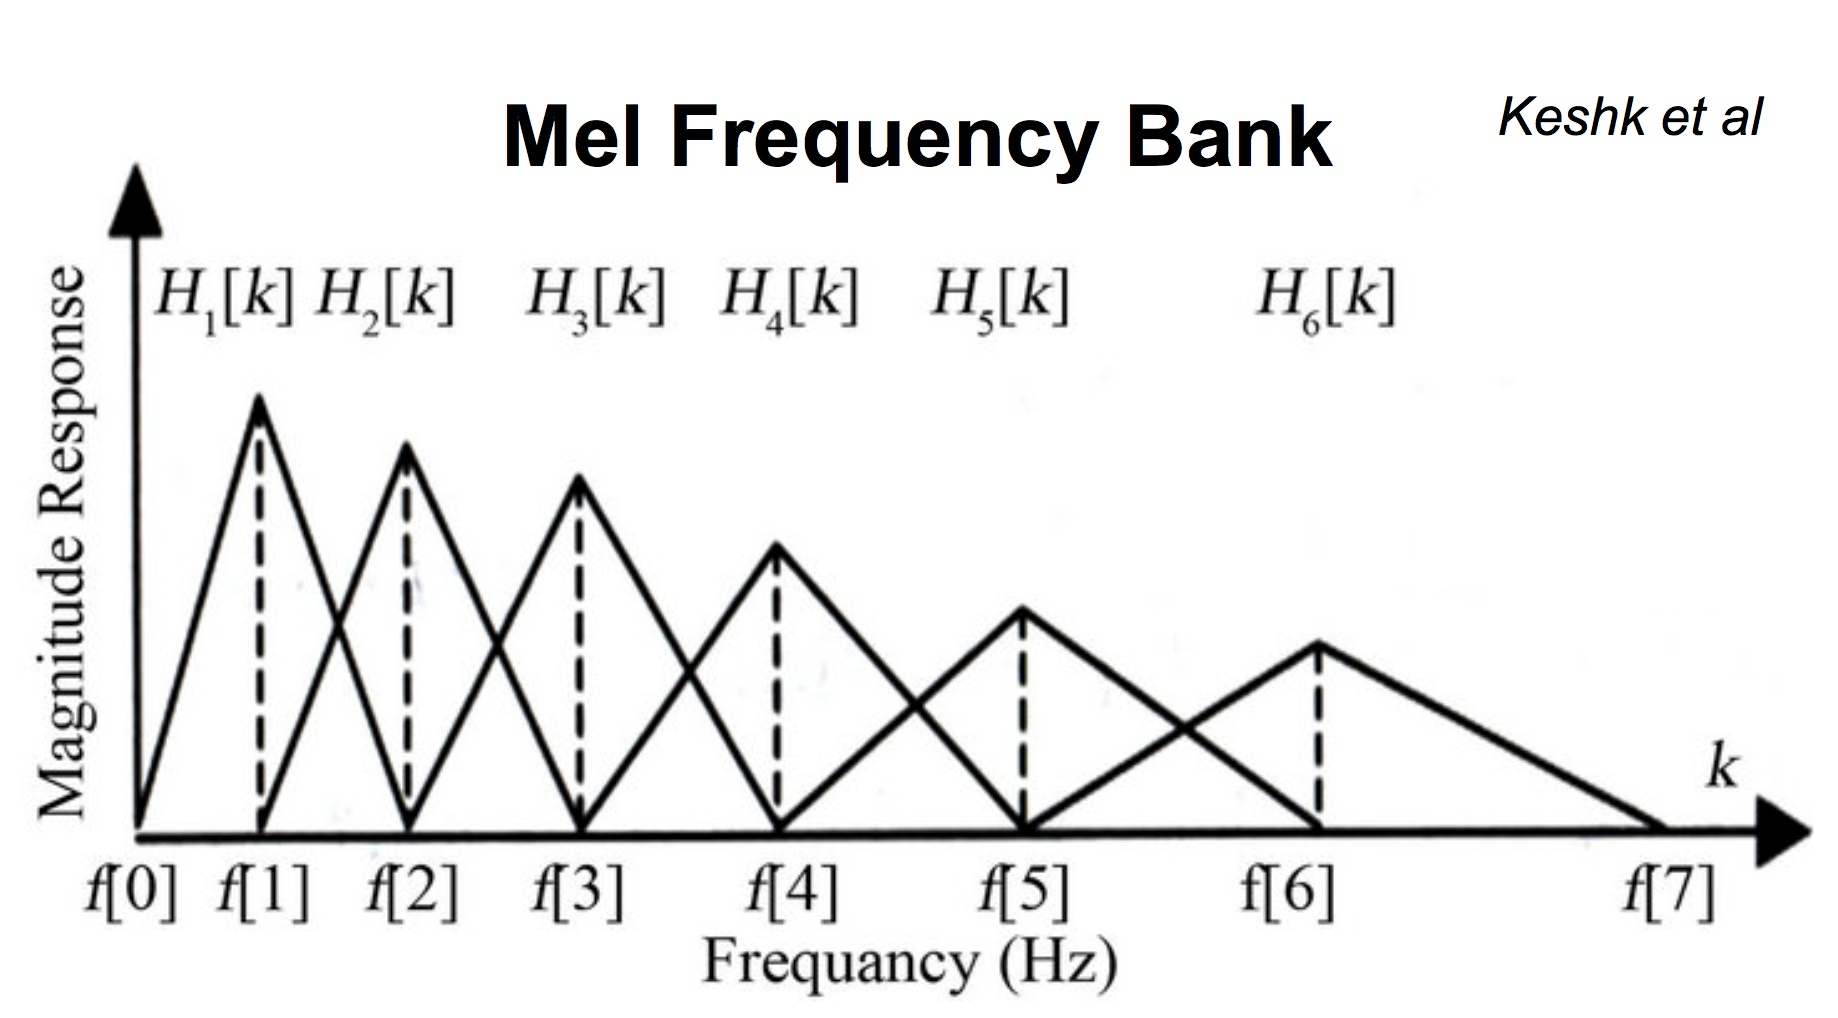
\includegraphics[width=8.5cm]{image6}}
%  \vspace{2.0cm}
\end{minipage}
% %
% \begin{minipage}[b]{.48\linewidth}
%   \centering
%   \centerline{\includegraphics[width=4.0cm]{image3}}
% %  \vspace{1.5cm}
%   \centerline{(b) Results 3}\medskip
% \end{minipage}
% \hfill
% \begin{minipage}[b]{0.48\linewidth}
%   \centering
%   \centerline{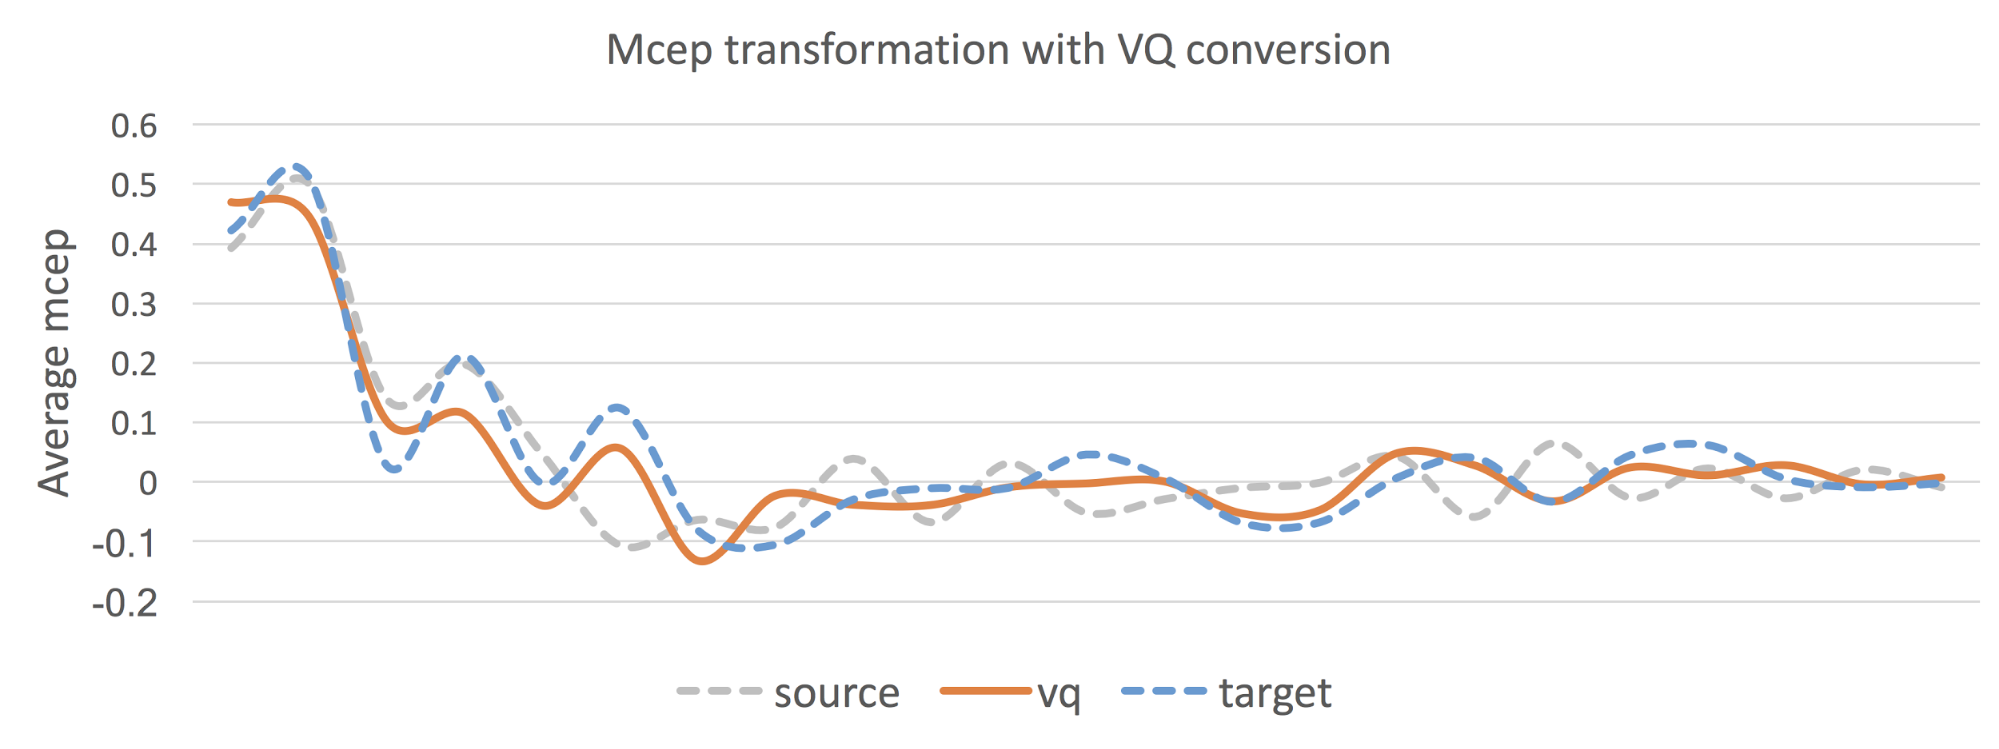
\includegraphics[width=4.0cm]{image4}}
% %  \vspace{1.5cm}
%   \centerline{(c) Result 4}\medskip
% \end{minipage}
% %
\caption{Mel frequency bank}
\label{fig:melfrequency}
%
\end{figure}

When using the Mel Frequency bank to imitate the human auditory response, first the Fourier Transform of the speech signal is taken to transform the signal to the time domain. Next, the Mel Frequency Bank is applied as a filter to the frequency-domain signal. Then the logarithm is taken across all frequencies to convert the spectrum into a dB scale. The frequencies are filtered out above 4 kHz, to keep only the voiced frequencies in the signal. Finally, the Discrete Cosine Transform is taken, converting the signal to Mel-Frequency Cepstral Coefficients (MFCC's), which will be referred to as Mel's cepstrum throughout this paper.

\subsection{Dynamic Time Warping}

Before feeding the features for training, target and source speaker's cepstrums should be aligned using Dynamic Time Warping(DTW), a nonlinear method of finding optimal alignment between two time-series data \cite{ratanamahatana2004everything}. The algorithm computes the matrix of distances between each two points, as shown below.
\begin{align*}
C_t = |mc^t_{source} - mc^t_{target}|
\end{align*}

\begin{figure}[htb]

\begin{minipage}[b]{1.0\linewidth}
  \centering
  \centerline{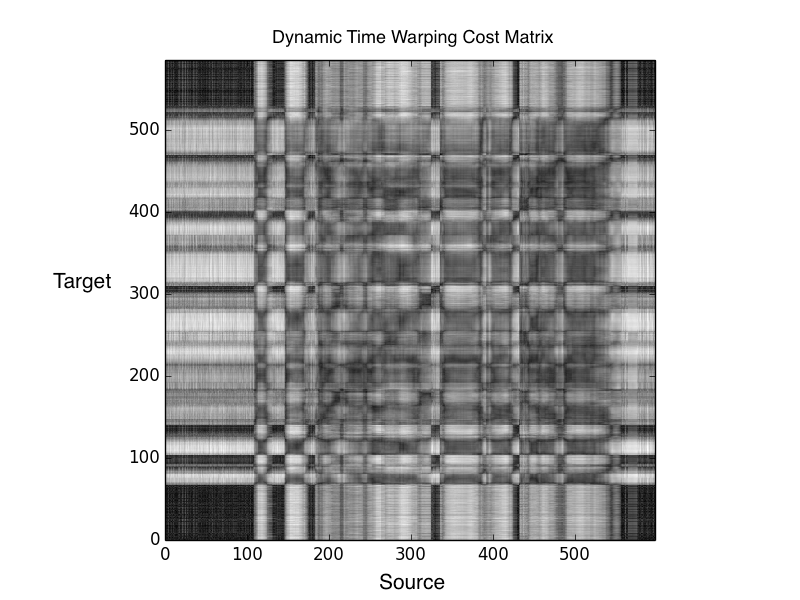
\includegraphics[width=8.5cm]{image9}}
%  \vspace{2.0cm}
\end{minipage}
\caption{The distance matrix between source and target data}
\label{fig:costmatrix}
%
\end{figure}

To discover the warp, it find the path through the matrix that minimizes the total cumulative distances between the two sequences. The algorithm is fairly straightforward. First, the (0,0) point’s value is kept the same. Then, it assigns each cell along the first column the running sum of the elements below it:
\begin{align*}
    D(0,m) = \sum_{k=0}^m c(0,y_k)
\end{align*}
Similarly, it assigns each cell along the first row the running sum of the elements before it.
\begin{align*}
    D(n,0) = \sum_{k=0}^n c(x_k,0)
\end{align*}
Finally, it iteratively selects the smallest value from the cells to the left, below, and diagonal left-below, summing that value with the value in the current cell.
\begin{align*}
    D(n,m) &= min\{D(n-1,m-1),D(n-1,m),D(n,m-1)\} \\
    &+c(x_n,y_m)
\end{align*}
This creates the accumulated cost matrix and allows for efficient calculation of the best path.

\begin{figure}[htb]

\begin{minipage}[b]{1.0\linewidth}
  \centering
  \centerline{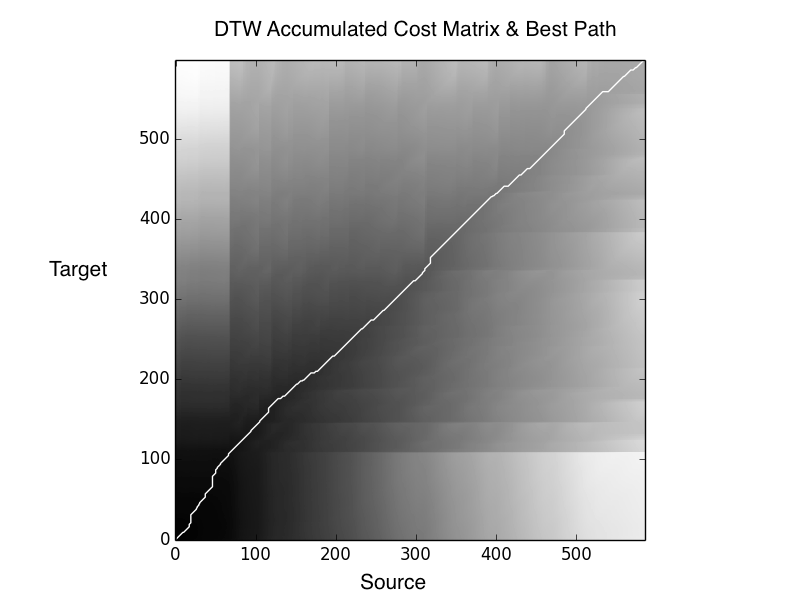
\includegraphics[width=8.5cm]{image10}}
%  \vspace{2.0cm}
\end{minipage}
\caption{The accumulated cost matrix and the best path}
\label{fig:accucostmatrix}
%
\end{figure}

\subsection{Gaussian Mixture Model}
A Gaussian Mixture Model represents the data as a weighted sum of Gaussian distributions, each with a characteristic mean and variance. Gaussian Mixture Models (GMMs) have been shown to be a reliable choice for voice conversion because Mel's cepstrums can be represented as a mixture of multiple Gaussian components\cite{stylianou1998continuous}. We will elaborate on their use in the next section.